\begin{minipage}{.34\textwidth}
    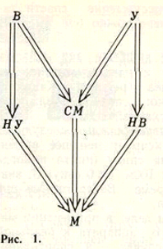
\includegraphics[width=140 pt]{images/2.png}
    \\
    \noindent
    \textbf{Ограниченность}
    \\
    К поняти \textit{ограниченной}
    после-довательности, введенному в учебни-ке (п.26), полезно добавить еще два: последовательность (\(x_n\)) называется \textit{ограниченной сверху}, если существу-ет такое число \(M\), всех \(n\)
    \[x_n \leq M;\]
    последовательность (\(x_n\)) называется \textit{ограниченной снизу}, если существу-ет такое число \(m\), что для всех n
    \[x_n \geq m.\]
    Очевидно, последовательность (\(x_n\)) тогда и только тогда является огра-ниченной,когда она ограничена свер-ху и снизу.
    \\ 
    
    \hspace{0.5cm}У п р а ж н е н и я

    \hspace{0.5cm}\textbf{5}. 
    \begin{tiny}
    Приведите четыре примера после-довательностей: ограниченной сверху, но не снизу; ограниченной снизу, но не сверху; не ограниченной ни снизу, ни сверху; ограниченной и снизу, и сверху.
    \end{tiny}
    
    \hspace{0.5cm}\textbf{6}. 
    \begin{tiny}
    Докажите, что любая неубывающая последовательность ограничена снизу, любая невозрастающая - сверху.
    \end{tiny}
    \\
    \\
    \textbf{Существование предела}
    
    \hspace{0.5cm}В учебнике доказывается, что \textit{если последовательность имеет предел, то она ограничена} (п. 26). Следовательно, \textit{если последовательность не ограничена, то она предела не имеет.}

    \hspace{0.5cm}Кроме того, в учебнике формулиру-ется упомянутая в начале статьи теорема Вейерштрасса: \textit{если последовательность монотонна и ограничена, то она имеет предел} (п. 32).

\end{minipage}
\hspace{0.5cm}
\begin{minipage}{.45\textwidth}
   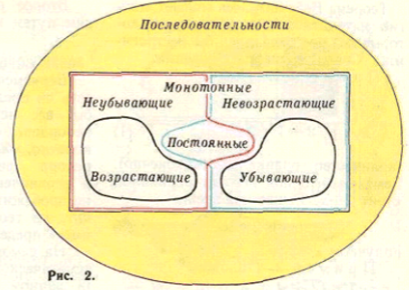
\includegraphics[width=300 pt]{images/3.png}
   \hspace{0.5cm}Ситуация станет более ясной, если мы изобразим ее в виде таблцы. Любая последовательность обладает (знак $+$ в таблице ниже) или не обладает (знак $-$) каждым из двух свойств, указанных в над <<входными>> стобцами таблицы. Таким образом, возникают четыре возможности. В трех случаях сформулированные выше теоремы позволяют утверждать существование (знак $+$ в <<выходном>> столбце таблицы) или несуществование(знак $-$) предела. В четвертом случае (тертья строка таблицы) ничего определенного сказать нельзя(см. упр. 7).

       \begin{center}
        \begin{tabular}{|@{\hspace{0.7em}}c@{\hspace{0.7em}}|@{\hspace{0.7em}}c@{\hspace{.1\textwidth}}|@{\hspace{.1\textwidth}}c@{\hspace{.1\textwidth}}|}
            \hline
             монотон- & ограни- & существова-\\
             ность & ченность & ние предела\\
             \hline
             &&\\
             + & + & +\\
             &&\\
             \hline
             &&\\
             + & $-$ & $-$\\
             &&\\
             \hline
             &&\\
             $-$ & + &  \\
             &&\\
             \hline
             &&\\
             $-$ & $-$ & $-$\\
             &&\\
             \hline
        \end{tabular}
    \end{center}
    
    \hspace{0.5cm}У п р а ж н е н и я
    
    \hspace{0.5cm}\textbf{7}. 
    \begin{tiny}
    Приведите пример немонотонной ограниченной последовательности, имеющей предел, и пример немонотонной ограни ченной последовательности, не имеющей предела.
    \end{tiny}
    
    \hspace{0.5cm}\textbf{8}. 
    \begin{tiny}
    Докажите, что последовательность 
    \[x_n = 1 + 2 + 3 + 4 ... +2^2\]не имеет прeделa.
    \end{tiny}
    \\\\\\\\\\
\end{minipage}